\documentclass{article}

\usepackage[utf8]{inputenc}     % for modern characters
\usepackage{microtype}          % for sexy kerning
\usepackage{tabularx}           % for wrapping tables
\usepackage{mathtools}          % for math
\usepackage{amssymb}            % for math
\usepackage{rotating}           % for sideways tables
\usepackage{diagbox}            % for that weird slash box in the table's corner
\usepackage{siunitx}            % always remember your units
\usepackage{hyperref}           % for cross-referencing and urls
\usepackage[nottoc]{tocbibind}  % for adding the references section to the TOC
\usepackage{mdwlist}            % for 'squishing' lists in figures
\usepackage{placeins}           % for \FloatBarrier
\usepackage{circuitikz}
\usepackage{framed}

\setcounter{tocdepth}{2}                            % sections and subsections in TOC
\newcolumntype{Y}{>{\centering\arraybackslash}X}    % wrapped centered table column

% title stuff
{
    \title{
        Mobile Autonomous Vehicle for Research in Intelligent Control \\
        (MAVRIC) \\
        \Large \emph{Preliminary Project Design Document}
    }
    \author{
        Chad Condon\thanks{
        Institute of Technology, University of Washington Tacoma} \\
        \url{ccondon@uw.edu}
        \and
        Keenan Fejeran\footnotemark[1] \\
        \url{kfejeran@uw.edu}
        \and
        Ben Foster\footnotemark[1] \\
        \url{benf94@uw.edu}
        \and
        Caleb Horst\footnotemark[1] \\
        \url{calebjh@uw.edu}
    }
    \date{March 17, 2015}
}

\begin{document}

% Title page
{
    \maketitle
    \thispagestyle{empty}
    \clearpage
}

% Front matter
{
    \pagenumbering{roman}
    \tableofcontents
    \clearpage
    \listoffigures
    \listoftables
    \clearpage
}

\setcounter{page}{1}
\pagenumbering{arabic}

\section{Problem Statement} %DONE (CC)
    \label{sec:problem_statement}

    Professor Mobus has a robotics platform for graduate research.
    Time and previous projects have created a need
    for updating and expanding its communication and control systems.
    The platform needs an on-board embedded Linux computer
    that can transceive data and control signals
    and execute Professor Mobus's learning algorithm.
    An ARM microcontroller will be used
    to interface with sensor arrays and actuators.
    Sensors are to be implemented to mimic the senses of a typical mammal.
    Existing power systems will be adapted
    to supply new and retained components
    with an aim to support uninterrupted 3+ hour experiments.
    Component selection, software choices, and design decisions
    need to be made with extensibility
    and the Bachelor of Science in Computer Engineering and Systems (CES) curriculum in mind.

\section{Background} %DONE (CC)
    \label{sec:background}

    Professor Mobus directs graduate research
    at the University of Washington Tacoma's Institute of Technology
    under the banner of his Adaptive Agents Laboratory\footnote{%
        \url{http://faculty.washington.edu/gmobus/AdaptiveAgents/}
    }.
    The lab is dedicated to the study of adaptive processes
    in artificial agents. Professor Mobus's Adaptrode learning mechanism%
    \cite{adaptrode}
    is an implementation of an artificial neural network
    which emulates animalian learning in a dynamic environment.

    Professor Moubus's
    Mobile Autonomous Vehicle for Research in Intelligent Control
    (MAVRIC)\cite{mavric}
    is the robotics platform used for testing of these adaptive agents.
    The MAVRIC began as a commercial ActivMedia Pioneer 2 platform.
    The platform maneuvered with two independently motorized wheels.
    It was powered by an on-board bay
    loaded with 1--3 \SI{12}{\volt} rechargeable batteries.
    Stimuli to the MAVRIC were delivered
    from nearby objects to a sonar array,
    from radio controlled lights to four light sensors, and
    from radio controlled speakers to a microphone.
    Processing was done remotely from a computer base station.

    Last year, a team attempted to modernize
    and extend the MAVRIC's sensing and computing platforms.\cite{mobot}
    The team succeeded in interfacing the motors and the sonar array.
    However, the team used two Arduino Mega microcontroller boards
    for discrete input and output processing
    and a Raspberry Pi single board computer (SBC) for higher level processing.
    Wiring was done using multiple breadboards and impermanent jumpers.
    The client was generally dissatisfied with the product.

    Moving forward, a more intentional, engineering driven design is expected.
    Professor Mobus would prefer architectures          %TODO: prefer or require?
    that fall in line with the Institute of Technology's curricula
    (e.g. ARM Cortex-M).
    This platform is intended for continued graduate research
    into adaptive agents and artificial intelligence.

    The team was motivated to pursue this project
    due to its larger scope and complexity.
    There is a strong interest in robotics, as well as graduate research,
    among our team.
    Compared to the others proposed,
    this project presented much more interesting problems and opportunities.

\FloatBarrier
\section{Design Plan} %DONE (CC)
    \label{sec:design_plan}

    Design began with analysis of the artifact's characteristics.
    These characteristics were identified
    and categorized as objectives, constraints, functions, and means.
    These are shown in Table~\ref{tab:characteristics}.
    The following subsections describe each of these categories more thoroughly.

    \begin{sidewaystable}
        \centering
        \begin{tabularx}{\textwidth}{|l||Y|Y|Y|Y|}
            \hline
            \textbf{Characteristic}
                & \textbf{Objective}
                & \textbf{Constraint}
                & \textbf{Functionality}
                & \textbf{Means}
            \\ \hline
            High resolution audio sensing
                & \checkmark
                & 
                & 
                & 
            \\ \hline
            Long battery life
                & \checkmark
                & 
                & 
                & 
            \\ \hline
            Low cost
                & \checkmark
                & 
                & 
                & 
            \\ \hline
            Small operating system
                & \checkmark
                & 
                & 
                & 
            \\ \hline
            Wide range audio sensing
                & \checkmark
                & 
                & 
                & 
            \\ \hline
            ``Curriculum compatible'' microcontroller and computer
                & 
                & 
                & 
                & \checkmark
            \\ \hline
            Uses existing sonar array
                & 
                & 
                & 
                & \checkmark
            \\ \hline
            Linux operating system
                & 
                & \checkmark
                & 
                & \checkmark
            \\ \hline
            Compatible with Adaptrode brain software
                & 
                & \checkmark
                & 
                & 
            \\ \hline
            Battery level monitor
                & 
                & \checkmark
                & \checkmark
                & 
            \\ \hline
            Drive motor control
                & 
                & \checkmark
                & \checkmark
                & 
            \\ \hline
            Senses distances to forward obstacles
                & 
                & \checkmark
                & \checkmark
                & 
            \\ \hline
            Wireless data transmission
                & 
                & \checkmark
                & \checkmark
                & 
            \\ \hline
            Wireless stop switch
                & 
                & \checkmark
                & \checkmark
                & 
            \\ \hline
            Cliff detection
                & 
                & 
                & \checkmark
                & 
            \\ \hline
            Touch sensor
                & 
                & 
                & \checkmark
                & 
            \\ \hline
            Gradient sensing to mimic smell
                & 
                & 
                & \checkmark
                & 
            \\ \hline
            Inertial sensing
                & 
                & 
                & \checkmark
                & 
            \\ \hline
            Interfaces with camera
                & 
                & 
                & \checkmark
                & 
            \\ \hline
            Internal cooling
                & 
                & 
                & \checkmark
                & 
            \\ \hline
            Internal temperature sensing
                & 
                & 
                & \checkmark
                & 
            \\ \hline
            Sound output
                & 
                & 
                & \checkmark
                & 
            \\ \hline
            Stereoscopic audio sensing
                & 
                & 
                & \checkmark
                & 
            \\ \hline
        \end{tabularx}
        \caption{Characteristics}
        \label{tab:characteristics}
    \end{sidewaystable}

    \subsection{Objectives}
    
        The following objectives were identified for the MAVRIC design.
        Measurable units and point values are assigned to each.
        Note that the points awarded for each objective
        fall within the range of 0--10.
        Any larger and smaller scores are mapped to 10 and 0 respectively.

        \subsubsection{Low Cost}
            The budget for the project is to be reasonably minimized.
            The client proposed a reasonable budget estimate of \$200.
            The unit  assigned to measure cost is dollar amount ($c$).
            This metric is weighted by the point assigning formula
            \begin{equation} \label{eq:cost}
                p = 400 -\frac{c}{30}.
            \end{equation}

        \subsubsection{Small Operating System}
        
            In order to provide for future extension of the project
            and to ensure system responsiveness,
            the size of the operating system is to be minimized.
            The size of the operating system is measured
            in gigabytes occupied on the file system ($f$).
            This metric is weighted by the point assigning formula
            \begin{equation}
                p = 12 - 4f.
            \end{equation}

        \subsubsection{Long Battery Life}
        
            The MAVRIC platform is intended for use
            in experiments lasting as long as three hours.
            As such the operation time for the robot on a single charged battery
            is to be maximized.
            Hours are the unit used to measure to time
            the robot functions on a single charged battery ($t$).
            Points for this objective are awarded by the formula
            \begin{equation}
                p = 5 t - 12.5.
            \end{equation}

        \subsubsection{Wide Range Audio Sensing}
        
            Audio sensing on the MAVRIC is intended
            to emulate an animal's hearing.
            As such, it should detect as much
            of the audible frequency range as feasible.
            The frequency range is gauged by octaves
            as determined by the maximum and minimum detectable frequency
            ($f_\text{max}$, $f_\text{min}$).
            Points for this objective are awarded by the formula
            \begin{equation}
                p = \log_2\left( \frac{f_\text{max}}{f_\text{min}} \right).
            \end{equation}

        \subsubsection{High Resolution Audio Sensing}
        
            The resolution of audio sensing is a measure
            of the granularity of the audio input.
            Sound within discrete frequency bands will be measured.
            As such, the number of these bands ($n$)
            is to maximized towards an ideal of 10.
            Points for this objective are awarded by the formula
            \begin{equation}
                p = 2n - 10.
            \end{equation}
    
    \subsection{Constraints}
        \label{sub:constraints}
        
        The following constraints were identified for the
        MAVRIC design. Some of these constraints were also
        identified as either functions (\ref{sub:functions}) or means.

        \subsubsection{Battery Level Monitor}
        
            A battery level monitor needs to be implemented
            in order to mimic ``hunger'' and to also keep track
            of how much power is left during an experiment.

        \subsubsection{Compatible with Adaptrode Brain Software}
        
            Graduate research students will be developing
            Adaptrode brain software for this robot.
            The software is written in C++
            and optimized for a Linux environment.
            Our hardware and software systems
            must be compatible with the Adaptrode brain software.

        \subsubsection{Drive Motor Control}
        
            The robot should be able to drive the motors in order to move about.
            This will be done with varying power
            so the vehicle can move at different speeds
            and turn at varying angles.

        \subsubsection{Linux Operating System}
        
            The single-board computer (SBC) on the MAVRIC
            must be running a distribution of Linux.

        \subsubsection{Senses Distances to Forward Obstacles}
        
            There is already an existing Sonar array mounted on the robot
            that is connected to a driver and functions properly.
            Therefore there is no need to replace this sonar array
            or fabricate our own.

        \subsubsection{Wireless Data Transmission}
        
            The MAVRIC collects data from its sensors during experiments.
            These data need to be sent wirelessly to the base station.

        \subsubsection{Wireless Stop Switch}
        
            A stop switch located on the base station
            needs to be able to halt all processes on the robot
            at any time during an experiment.
            This is to prevent any damage that may be caused to the vehicle or surrounding environment 
            and this is a way to halt the experiment
            if there is any unpredicted behavior.

    \subsection{Functions}
        \label{sub:functions}
        
        The following functions of the MAVRIC were identified.
        Some of these were also recognized as constraints
        discussed previously in~\ref{sub:constraints}.
        Performance specifications for each of the functions were created.
        Candidate means for each of these functions were also generated
        and are compared in Table~\ref{tab:morphchart}.

        \subsubsection{Battery Level Monitor}
        
            The MAVRIC will be able to gauge the charge level of its battery.
            During experiments, this data will serve as an analog to hunger.

        \subsubsection{Drive Motor Control}
        
            The MAVRIC will maneuver using two independently driven DC motors.
            Control signals for these motors will be passed
            from the brain software.

        \subsubsection{Gradient Sensing to Mimic Smell}
        
            In order to simulate smell,
            the MAVRIC will have continuous sensor input
            representing discrete ``odor'' signals.
            These signals are to be generated from beacons in the environment
            such that signal readings increase with proximity to the beacon.

        \subsubsection{Inertial Sensing}
        
            In order to simulate an animal's vestibular system,
            inertial sensing will be implemented.
            Readings from the three lateral or rotational axes
            are acceptable.

        \subsubsection{Interfaces with Camera}
        
            To provide for extension of the MAVRIC's capabilities
            and future research into computer vision,
            a color video camera is to be installed.
            The camera will not be utilized in the current scope of this project.

        \subsubsection{Internal Cooling}
        
            As a mammal does by sweating,
            the MAVRIC will be able to cool itself.
            The ActivMedia Pioneer 2 platform has an internal fan
            which may be utilized.

        \subsubsection{Internal Temperature Sensing}
        
            The MAVRIC will monitor its internal temperature.
            This data will be provided to the brain software
            for interpretation.

        \subsubsection{Senses Distances to Forward Obstacles}
        
            The MAVRIC will sense physical obstacles
            within a short range of its front.
            This sense is to emulate an animal's antennae.
            The ActivMedia Pioneer 2 platform includes a sonar array
            which may be utilized.

        \subsubsection{Sound Output}
        
            The MAVRIC will be capable of generating different sounds.
            The ActivMedia Pioneer 2 platform includes a small speaker
            which may be utilized.

        \subsubsection{Stereoscopic Audio Sensing}
        
            To emulate hearing, the MAVRIC will have two audio sensors
            which will be used to create level readings
            within discrete audible frequency bands.
            These signal filters will need to be developed and implemented.

        \subsubsection{Wireless Data Transmission}
        
            The Adaptrode brain software interprets data and generates signals
            through ``in-slots'' and ``out-slots.''
            During experiments, these data will be transmitted wirelessly
            to a computer base station for logging and analysis.

        \subsubsection{Wireless Stop Switch}
        
            Functionality for remotely pausing operating of the robot
            will be provided.
            This will allow for a ``kill switch''
            for service to the robot or environment
            during an ongoing experiment.

        \begin{sidewaystable}[htb]
            \centering
            \begin{tabularx}{\textwidth}{|X||Y|Y|Y|Y|}
                \hline
                \backslashbox{Functions}{Means}
                    & 1
                    & 2
                    & 3
                    & 4
                \\ \hline
                Battery Level Monitor
                    & Voltage divider to ADC
                    &
                    &
                    &
                \\ \hline
                Drive Motor Control
                    & Pololu drivers
                    & Alternate driver
                    &
                    &
                \\ \hline
                Gradient Sensing To Mimic Smell
                    & Filtered light-to-frequency sensors
                    & Filtered photoresistors
                    & Filtered audio
                    & Bluetooth
                \\ \hline
                Inertial Sensing
                    & Accelerometer
                    & Gyro
                    & Dual package
                    &
                \\ \hline
                Internal Cooling
                    & Motor driver and fan
                    & Op-amp and fan
                    & Transistor amp and fan
                    &
                \\ \hline
                Internal Temperature Sensing
                    & Thermistor and voltage divider
                    & Tiva internal sensor
                    & Thermocouple
                    &
                \\ \hline
                Senses Distances to Forward Obstacles
                    & Microcontroller driven sonar
                    & Raspberry Pi driven sonar
                    &
                    &
                \\ \hline
                Sound Output
                    & SBC output with amplifier
                    & single frequency tones from microcontroller
                    &
                    &
                \\ \hline
                Stereoscopic Audio Sensing
                    & hardware filters
                    & SDFT
                    & FFT
                    & Goetzel algorithm \\ \hline
                Wireless Data \mbox{Transmission}
                    & XBee
                    & Wi-Fi
                    &
                    &
                \\ \hline
                Wireless Stop Switch
                    & integrated into data transmission
                    & exclusive interface
                    &
                    &
                \\ \hline
                Interfaces with \mbox{Camera}
                    & Raspberry Pi camera
                    & COTS camera
                    &
                    &
                \\ \hline
                Touch Sensor
                    & button bumpers
                    & pressure pads
                    & flex sensors
                    & custom sensor
                \\ \hline
                Cliff Detection
                    & ultrasonic to main microcontroller
                    & IR to main microcontroller
                    & ultrasonic to slave microcontroller
                    & IR to main microcontroller
                \\ \hline
                Interchip \mbox{Communication}
                    & I\textsuperscript{2}C
                    & SPI
                    & UART
                    &
                \\ \hline
            \end{tabularx}
            \caption{Morphological Chart}
            \label{tab:morphchart}
        \end{sidewaystable}

\FloatBarrier
\section{Design Research} %TODO
    \label{sec:design_research}
    
    % Summary of devices currently available
    The product being created is a specialized research platform, specifically
    outfitted with sensors and actuators for our clients desires.
    The chassis being retrofitted was originally a Pioneer 2 robot platform from ActivMedia.
    Other research platforms are available from Activrobots, such as the newer
    Pioneer III\footnote{\url{http://activrobots.com/ResearchRobots/PioneerP3DX.aspx}}
    and PeopleBot\footnote{\url{http://activrobots.com/ResearchRobots/PeopleBot.aspx}}. 
    % Evaluation of these devices for suitability in this project
    These platforms also have extra sensor arrays,
    however they do not have as much customizability as needed to implement all
    the desired functions.
    Furthermore, these packages come at a significant price,
    while the current project recycles resources to minimize cost.
    
    The Washington company CoroWare also produces
    a number of robotics platforms for research.%
    \footnote{\url{http://www.corobot.net/products/}}
    However, cost ranges from \$400\footnote{\url{http://www.corobot.net/spark/}}
    to \$19,999\footnote{\url{http://www.corobot.net/corobot-pro/}},
    well above the acceptable budget for the entire project.
    All of the platforms offered would also require significant adjustments
    and extension to meet the client's needs.
    
    %howzzat? As a starting point...

\FloatBarrier
\section{Design Alternatives} %TODO
    \label{sec:design_alternatives}
    
    % Details and drawings of each alternative
    % Consideration of constraints
    % How well do designs meet objectives (evaluate the metrics)
    % How well do designs meet functional requirements
    % Method for choosing among designs
    
    \subsection{Interchip Communication}
    
        The interchip communication
        (between the microcontroller and the SBC)
        has been identified as the project's \emph{high risk item}.
        The entire success of the project rests
        on effective, timely data transfer between these two
        processing platforms.
        The bulk of sensor data and actuator control
        will be driven by the microcontroller,
        but high level control will be done in
        Professor Mobus's brain software as installed on the SBC.
    
        \subsubsection{Universal Asynchronous Receiver/Transmitter}
        
            Serial communication using universal asynchronous receiver/transmitter
            (UART) is perhaps the simplest approach.
            However, because we chose to use the XBee for wireless data transmission,
            the serial resource needed to use UART is unavailable.
            
        \subsubsection{Serial Peripheral Interface}
            
            Serial peripheral interface (SPI)
            is a solution that uses $3 + N$ wires
            for synchronous communication between a master and $N$ slaves.
            Research suggests that SPI is less of an industry standard
            compared to I\textsuperscript{2}C.
            In addition SPI requires more resources to expand upon
            if more slave nodes were desired. These aspects cause an otherwise
            practical solution to score poorly amongst other choices.
        
    \subsection{Base Station Communication} % DONE (BF)
        \label{sub:base_station_communication}
        
        Communication between the robot and the base station was a
        relatively easy decision to make since we were provided an Xbee
        and found that it fit our needs quite nicely.
        One other option was considered for sending data 
        back and forth between the robot and the base station. 
        
        \subsubsection{Wi-Fi}
            
            We considered plugging a USB Wi-Fi adapter into the Raspberry Pi
            and having it send data to the base station.
            That way we would have use of the serial port on the Raspberry Pi for
            UART interchip communication.
            Wi-Fi would also require reconfiguration for any given computer
            base station and create a compatiblity requirement
            between the two network adapters.
            The XBee, however, uses a similar means of communication
            and, while the Xbee is using the only serial port on the Raspberry Pi,
            it is still simpler to use than a Wi-Fi communication device
            and it serves its purpose effectively without any recurring configuration.
    
        
    \subsection{Audio Input} %DONE (CC)
        \label{sub:audio_input_options}
        
        Multiple options were considered based on their fulfillment of
        the objectives of a wide total range of frequencies detectable
        and a large number of sub-ranges measured.
        
        \subsubsection{Hardware Solutions}
        
            A hardware solution would minimize the processing load of this filter
            at the cost of extensibility and configurability.
            
            \paragraph{Hardware Band-Pass Filters}
            
                The advantages provided by the use of hardware band-pass filters
                (as shown in Figure~\ref{fig:band-pass_filter})
                include its extensibility.
                By adding hardware,
                many ranges, bands and frequencies are possible.
                However,
                limited analog inputs on a microcontroller would
                require additional considerations or
                multiplexers or other hardware, tuning frequency ranges
                properly may be difficult or unfeasible, quantity of
                hardware necessary would make extension less elegant
                and wiring prone to error.
                
                \begin{figure}[htb]
                    \centering
                    \begin{circuitikz}[american voltages]
                        \draw
                        (0,0) to[sinusoidal voltage source, l^=microphone] (0,3)
                            to[resistor, l^=$R_1$] (3,3)
                            to[capacitor, l^=$C_1$] (3,0)
                        (3,3) to[capacitor, l^=$C_2$] (6,3)
                            to[resistor, l_=$R_2$, v^<=$v_\text{out}$] (6,0)
                            -- (0,0)
                        ;
                    \end{circuitikz}
                    \caption{Band-Pass Filter}
                    \label{fig:band-pass_filter}
                \end{figure}
        
            \paragraph{External Chips (MSGEQ7)}
        
                A discrete component such as this would provide an easy interface.
                An IC is a small package which saves space.
                This specific package also requires only minimal tuning.
                This solution would also require minimal processor time
                on either the microcontroller or the SBC.
                However, this solution would not provide for extensibility
                and only provides seven frequency bands.
        
        \subsubsection{Software Solutions}
        
            A software solution would allow for extensibility
            at the cost of a significant computational overhead.
        
            \paragraph{Fast Fourier Transform}
        
                A fast Fourier Transform (FFT) would provide a degree
                of extensibility and configurability
                in that it allows for arbitrarily defined bands.
                However, its use would require a large amount
                of high speed sampling requiring higher processor use.
                Also, the  team possesses limited practice in signal processing.
        
            \paragraph{Sliding Discrete Fourier Transform}
        
                A sliding discrete-time Fourier transform (SDFT)
                provides all of the functionality of the FFT
                at a smaller scale.
                However, it suffers from similar drawbacks as well.
        
            \paragraph{Goertzel Algorithm}
        
                The Goertzel algorithm provides a more numerically efficient approach
                to the Fourier transform.
                However this efficiency advantage is only at small numbers
                of frequencies.
                Also, the algorithm only measures specific frequencies,
                not bands.

\clearpage
\FloatBarrier
\section{Preliminary Design} %TODO
    \label{sec:preliminary_design}
    % Detailed description of chosen design
    % Requirements and Functional Specifications for chosen design

    Of the design choices discussed in Sections~\ref{sec:design_research}
    and~\ref{sec:design_alternatives},
    choices were made based on the parameters discussed in~\ref{sec:design_plan}
    and based on the feasibility of completing them within the alloted time
    and skill set of the team.
    Figure~\ref{fig:schematic} shows the preliminary electrical hardware design.
    
    The main computational platforms selected are the
    Texas Instruments Tiva C Series TM4C1294 LaunchPad%
    \footnote{\url{http://www.ti.com/ww/en/launchpad/launchpads-connected-ek-tm4c1294xl.html}}
    and the Raspberry Pi B+%
    \footnote{\url{http://www.raspberrypi.org/products/model-b-plus/}}.
    The Tiva was selected because it is the platform
    used in the CES curriculum
    and thus best satisifies curriculum compatibility.
    The Raspberry Pi B+ was chosen
    for its known compatibility with existing software
    and its improvements to the previous version's
    power and data busses.
    The new Raspberry Pi 2 B was not chosen
    because documentation and support for the upgraded ARMv7 processor
    are still immature.
    
    Alternatives to the Raspberry Pi, such as
    the BeagleBone Black\footnote{\url{http://beagleboard.org/BLACK}}
    and the CubieTruck\footnote{\url{http://cubieboard.org/model/cb3/}},
    were also considered.
    However they did not offer advantages significant enough
    to justify a change in platform.
    
    For interboard communication,
    the I\textsuperscript{2}C protocol was selected.
    This choice was deemed most appropriate
    because of its minimal wiring, high speed,
    and hardware support from both boards.
    
    Several hardware components from the existing platform are being retained.
    The sonar array completely satisfies the obstacle detection functionality.
    Its use will also reduce engineering time and cost.
    The original motors in the ActivMedia Pioneer 2 chassis
    are also being kept as they perform adequately.
    The stock battery bay satisfies the power requirements for the system.
    The motor drivers installed by last year's team%
    \footnote{\url{https://www.pololu.com/product/1451}}
    , the original fan,
    and the speaker are all likewise being used.
    
    Steroscopic audio sensing will be implemented
    using electret microphones%
    \footnote{\url{https://www.adafruit.com/products/1063}}
    and the MSGEQ7 graphic equalizer display filter%
    \footnote{\url{https://www.sparkfun.com/datasheets/Components/General/MSGEQ7.pdf}}.
    Though this solution only provides seven bands of resolution,
    the MSGEQ7 covers sufficient frequency range
    and off-boards all signal processing.
    Given the timing requirements of the microcontroller's software
    and the limited analog input capabilities of the Raspberry Pi,
    this compromise is deemed acceptable.
    This configuration requires minimal calibration, processing time,
    and physical space in the system.
    
    \begin{figure}[h!tb]
        \centering
        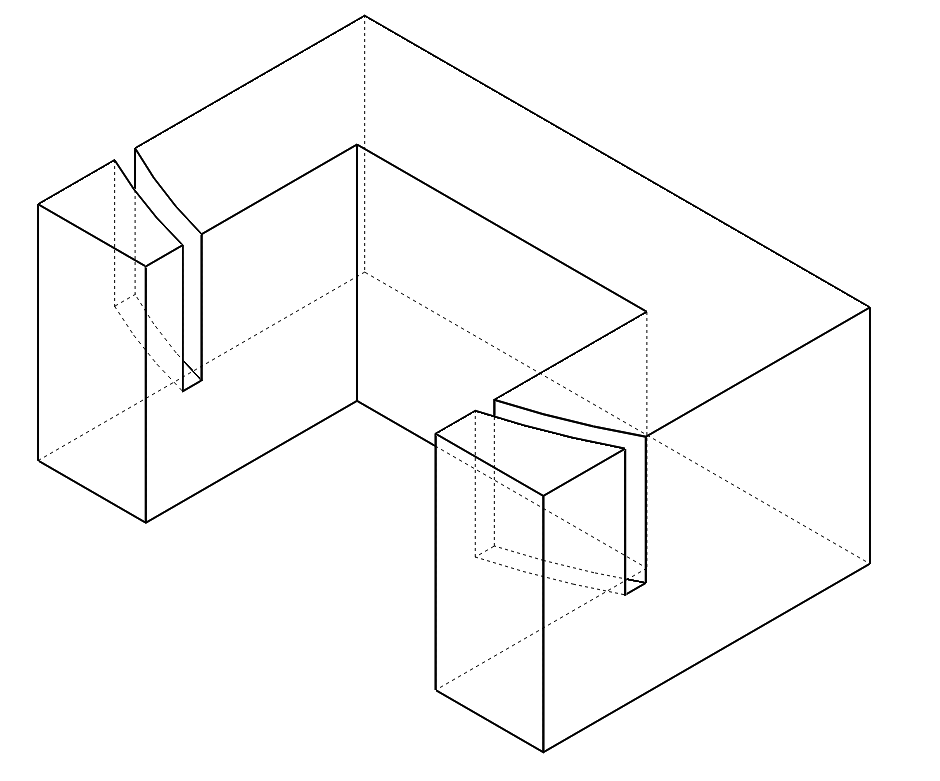
\includegraphics[width=.75\textwidth]{mount.png}
        \caption{Flex Sensor Bumper Mount}
        \label{fig:mount}
    \end{figure}
    
    Touch sensing will be implemented with flex sensors mounted offset
    from the perimeter of the chassis.
    The sensors operate as a variable resistor
    and will be configured with a voltage divider for input
    into the microcontroller's analog-to-digital converter (ADC).
    This layout is shown in  Figure~\ref{fig:schematic}.
    This design will create a continuous output signal
    as opposed to the binary output of a simple switch.
    This is more compatible with the client's anticipated use.
    Four sensors will be installed: one on each side and two in the rear.
    Front touch sensors are deemed redundant with the sonar array
    and have been excluded.
    Mounting hardware for the flex sensors will be modeled
    with SolidWorks and fabricated with an additive 3D printer
    at a local maker space.
    Figure~\ref{fig:mount} shows a design for the sensor mount.

    \begin{sidewaysfigure}[htb]
        \centering
        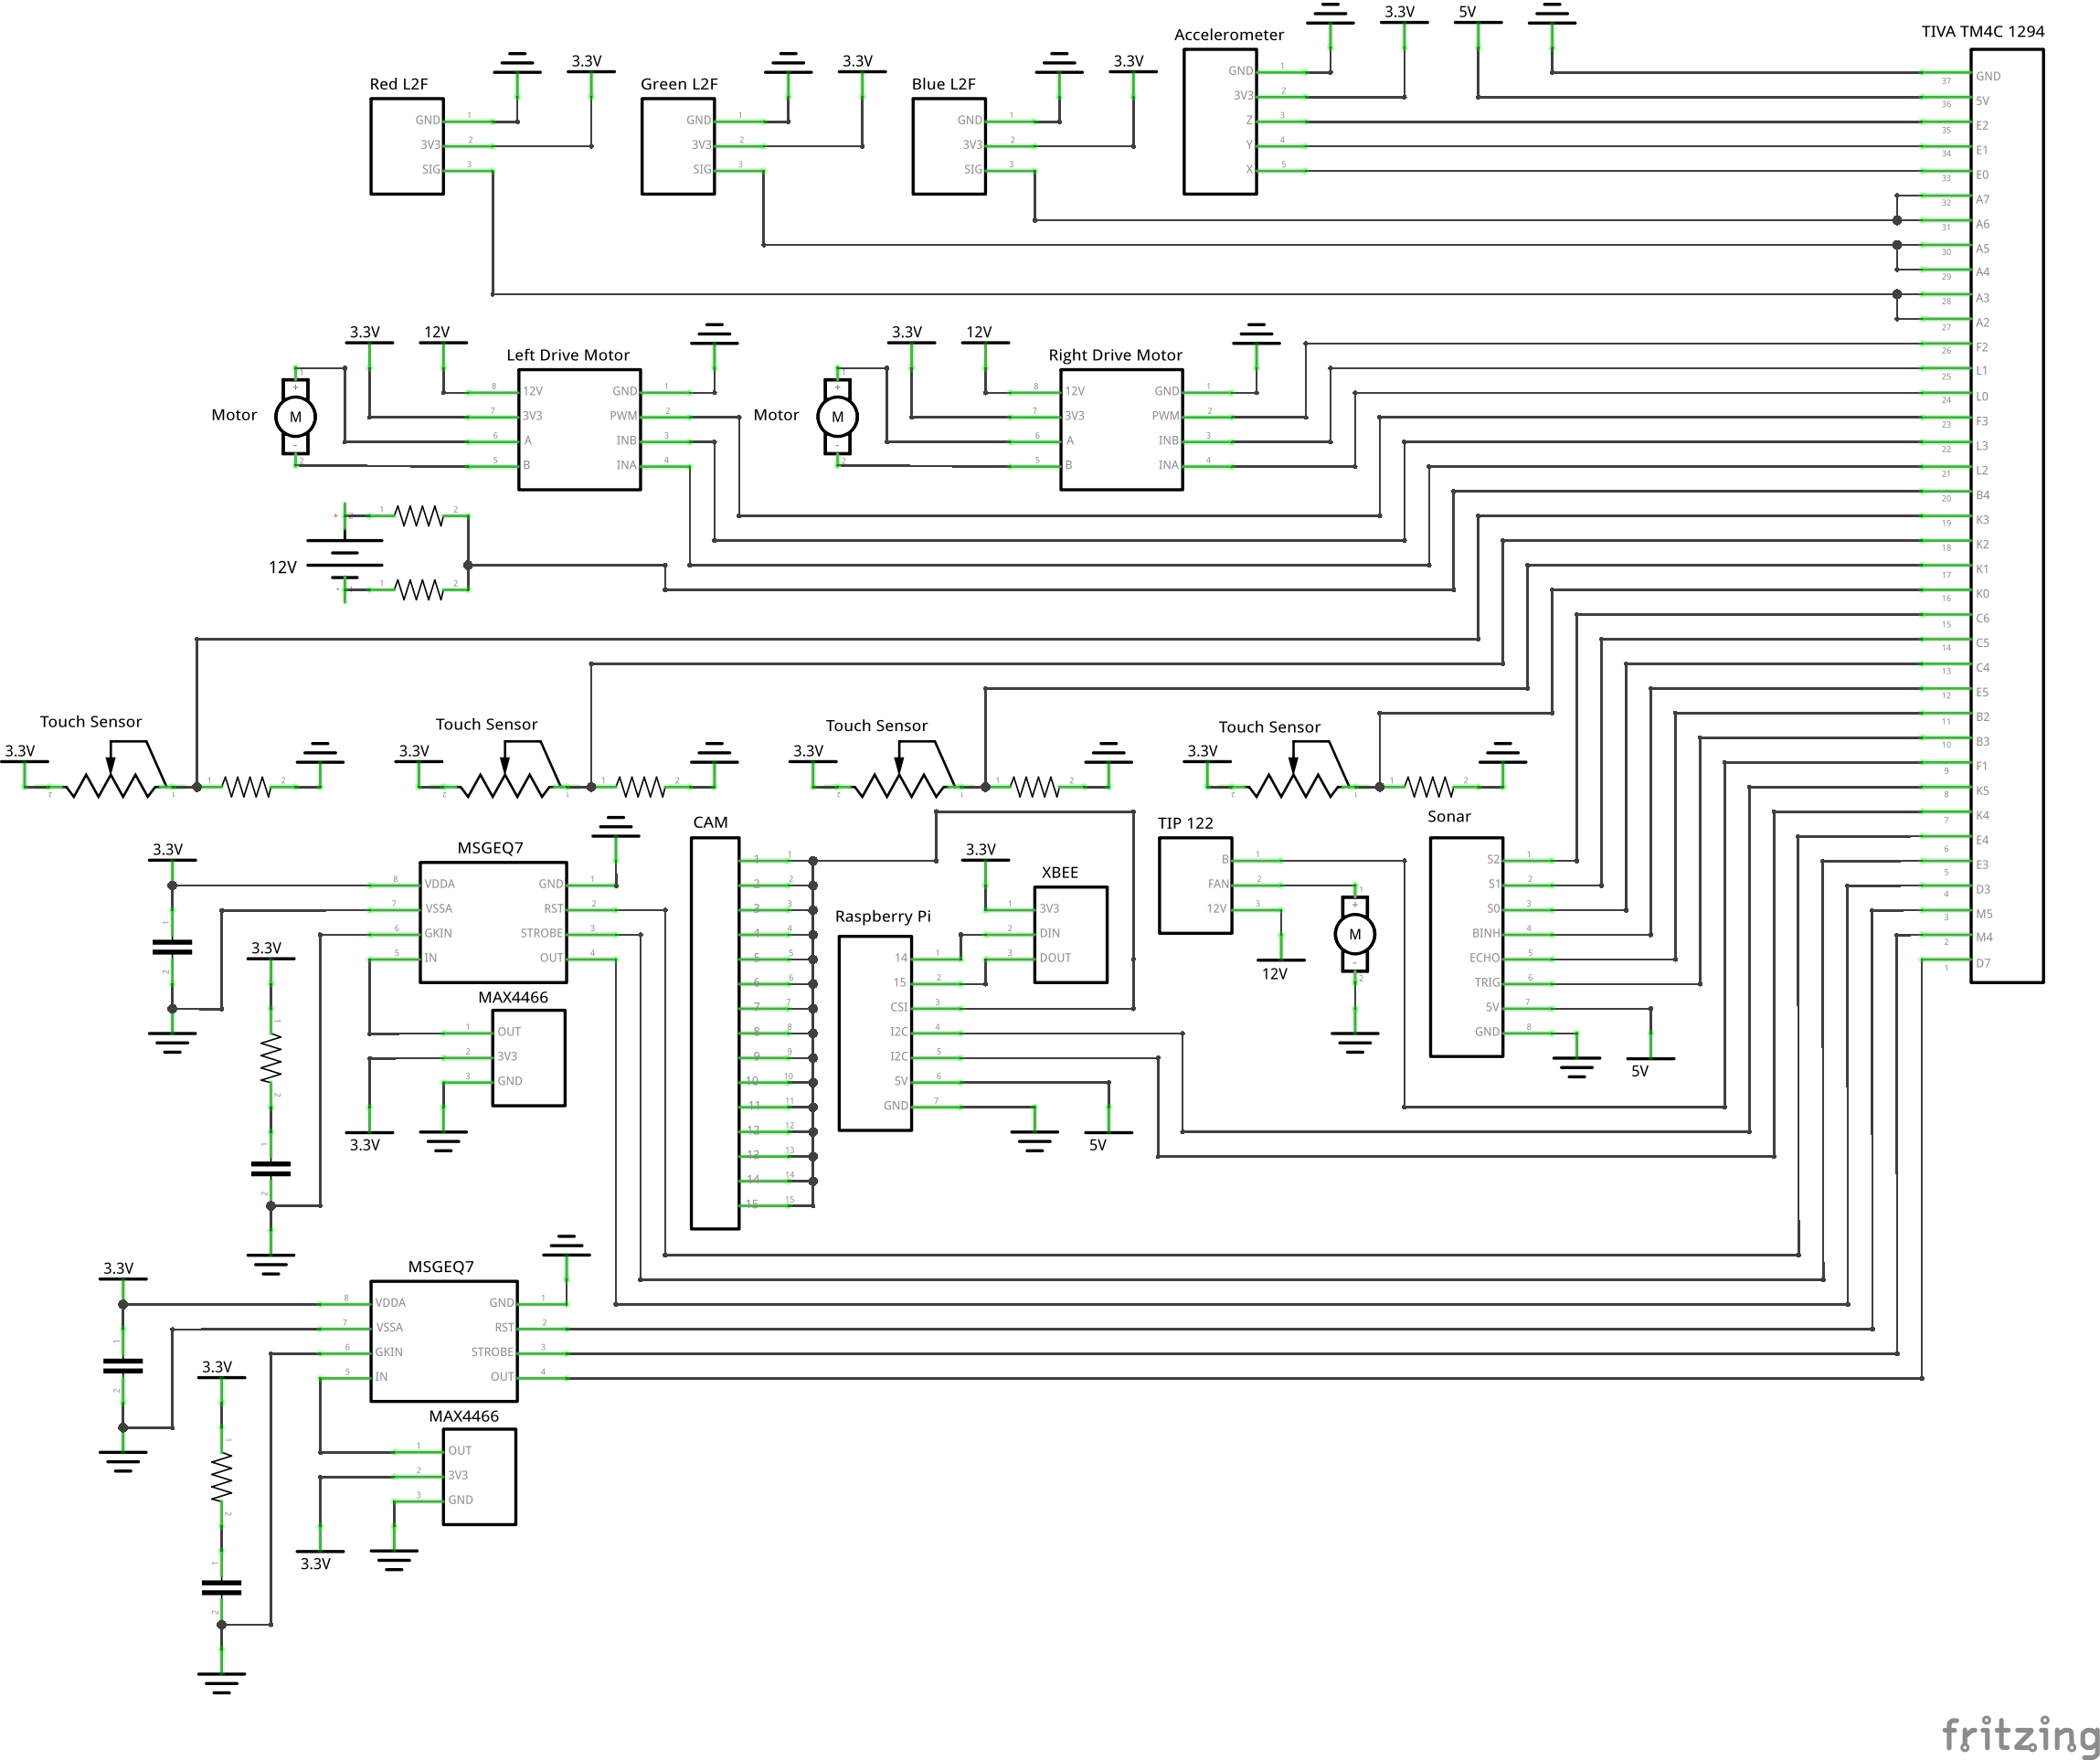
\includegraphics[width=\textwidth]{schematic.png}
        \caption{Electrical Schematic}
        \label{fig:schematic}
    \end{sidewaysfigure}
    
\FloatBarrier
\section{Testing} %DONE (CC)
    \label{sec:testing}
    
    Testing will be completed at every functional level of design.
    Unit testing will be done as each of the sub-components
    is fabricated or obtained to ensure anticipated behavior
    under our specified operating ranges.
    
    After system components are completed and tested,
    subsystems (such as those shown in Figure~\ref{fig:schematic})
    will be assembled from them.
    Integration testing will be done to ensure the expected interface.
    Likely flaws and failures will be identified
    and design revision will be required.
    The following test scripts demonstrate the type of unit testing
    that will be conducted.
    
    Figure~\ref{fig:hardware_script} shows the plan for hardware testing
    of the sonar array that has been developed.
    This testing is under way.
    Table~\ref{tab:sonar_data} shows the data collected in a single trial.
    These data are graphed in Figure~\ref{fig:sonar_results}.
    Further trials will increase the fidelity of the time-distance relationship
    and may correct for some experimental inconsistencies.
        
    \begin{figure}[htb]
        \centering
        \begin{framed}
        \begin{enumerate*}
            \item Using DC power supply at \SI{5}{\volt}
            \begin{enumerate*}
                \item Supply to sonar array
                \begin{enumerate*}
                    \item HIGH to \SI{5}{\volt}
                    \item GND to ground
                \end{enumerate*}
                \item Apply select signals to $S_2$, $S_1$, $S_0$
                as shown in Table~\ref{tab:sonar_select}
            \end{enumerate*}
            \item Using function generator
            \begin{enumerate*}
                \item Apply a \SI{3.3}{\volt} \SI{560}{\milli\second} pulse
                at \SI{10}{\hertz} to $TRIG$
                \item Apply a \SI{3.3}{\volt} \SI{560}{\milli\second} pulse
                at \SI{10}{\hertz} to \SI{570}{\milli\second} out of phase to $BINH$
            \end{enumerate*}
            \item Using oscilloscope
            \begin{enumerate*}
                \item Apply digital channel 0 probe to $TRIG$
                \item Apply digital channel 1 probe to $ECHO$
            \end{enumerate*}
            \item Position selected sonar sensor on ledge
            to prevent surface interference
            \item Using a ruler and object with a flat vertical surface
            \begin{enumerate*}
                \item Place the object such that its surface is orthogonal
                to the sensor
                \item Distance the object beginning at \SI{10.0}{\centi\meter}
                and incrementing by \SI{1.0}{\centi\meter} until
                \SI{40.0}{\centi\meter}
                \item Record the distance
            \end{enumerate*}
            \item Using the oscilloscope
            \begin{enumerate*}
                \item Measure and record the time between the rising edges
                on channel 0 and channel 1
            \end{enumerate*}
            \item Repeat 8 times for each sensor and populate data
            as shown in Table~\ref{tab:sonar_format}
        \end{enumerate*}
        \end{framed}
        \caption{Sonar Array Test Script}
        \label{fig:hardware_script}
    \end{figure}

    \begin{table}[htb]
        \centering
        \begin{tabular}{|c|c|c|c|}
            \hline
            $S_2$
                & $S_1$
                & $S_0$
                & \textbf{Sensor}
            \\ \hline
            0 & 0 & 0 & 1 \\ \hline
            0 & 0 & 1 & 0 \\ \hline
            0 & 1 & 0 & 3 \\ \hline
            0 & 1 & 1 & 2 \\ \hline
            1 & 0 & 0 & 5 \\ \hline
            1 & 0 & 1 & 4 \\ \hline
            1 & 1 & 0 & 7 \\ \hline
            1 & 1 & 1 & 6 \\ \hline
        \end{tabular}
        \caption{Sonar Select Signals}
        \label{tab:sonar_select}
    \end{table}

    \begin{table}[htb]
        \centering
        \begin{tabular}{|c|c|c|c|c|c|c|}
            \hline
            \textbf{$S_2$}
                & \textbf{$S_1$}
                & \textbf{$S_0$}
                & \textbf{Sensor}
                & \textbf{Object distance (\si{\centi\meter})}
                & \textbf{Trial}
                & \textbf{Time (\si{\milli\second})}
            \\ \hline
            0 & 0 & 0 & 1 & 10.0 & 1 & --- \\ \hline
            \ldots
                & \ldots
                & \ldots
                & \ldots
                & \ldots
                & \ldots
                & \ldots \\ \hline
            1 & 1 & 1 & 6 & 40.0 & 8 & --- \\ \hline
        \end{tabular}
        \caption{Sonar Test Data Format}
        \label{tab:sonar_format}
    \end{table}
    
    \begin{table}[htb]
        \centering
        \begin{tabular}{|r|llllllll|}
\hline
    \textbf{Distance (\si{\centi\meter})}    & \multicolumn{8}{c|}{\textbf{Time (\si{\milli\second})}}            \\
    \textbf{Sensor}    & \multicolumn{1}{c}{\textbf{0}}  & \multicolumn{1}{c}{\textbf{1}}     & \multicolumn{1}{c}{\textbf{2}}     & \multicolumn{1}{c}{\textbf{3}}     & \multicolumn{1}{c}{\textbf{4}}     & \multicolumn{1}{c}{\textbf{5}}     & \multicolumn{1}{c}{\textbf{6}}     & \multicolumn{1}{c|}{\textbf{7}}     \\ \hline
    10.0                            & 0.790     & 0.736 & 0.796 & 0.788 & 0.956 & 0.964 & 0.956 & 0.950 \\
    11.0                            & 0.800     & 0.744 & 0.792 & 0.792 & 0.956 & 0.960 & 0.948 & 0.950 \\
    12.0                            & 0.800     & 0.742 & 0.800 & 0.792 & 0.960 & 0.956 & 0.948 & 0.950 \\
    13.0                            & 0.800     & 0.736 & 0.812 & 0.800 & 0.960 & 0.956 & 0.968 & 0.970 \\
    14.0                            & 0.830     & 0.758 & 0.804 & 0.832 & 0.968 & 0.964 & 0.972 & 0.970 \\
    15.0                            & 0.880     & 0.828 & 0.880 & 0.888 & 0.972 & 0.972 & 1.03  & 1.04  \\
    16.0                            & 0.930     & 0.884 & 0.932 & 0.948 & 1.03  & 1.01  & 1.09  & 1.09  \\
    17.0                            & 0.990     & 0.940 & 0.996 & 1.01  & 1.09  & 1.09  & 1.14  & 1.15  \\
    18.0                            & 1.05      & 1.01  & 1.05  & 1.07  & 1.14  & 1.14  & 1.21  & 1.20  \\
    19.0                            & 1.11      & 1.07  & 1.11  & 1.13  & 1.20  & 1.20  & 1.26  & 1.26  \\
    20.0                            & 1.19      & 1.13  & 1.18  & 1.19  & 1.27  & 1.25  & 1.32  & 1.31  \\
    21.0                            & 1.24      & 1.19  & 1.33  & 1.26  & 1.32  & 1.32  & 1.37  & 1.37  \\
    22.0                            & 1.29      & 1.25  & 1.39  & 1.32  & 1.38  & 1.37  & 1.43  & 1.43  \\
    23.0                            & 1.36      & 1.31  & 1.45  & 1.38  & 1.44  & 1.43  & 1.49  & 1.49  \\
    24.0                            & 1.41      & 1.37  & 1.51  & 1.44  & 1.50  & 1.49  & 1.54  & 1.55  \\
    25.0                            & 1.46      & 1.48  & 1.57  & 1.49  & 1.55  & 1.55  & 1.61  & 1.61  \\
    26.0                            & 1.53      & 1.54  & 1.63  & 1.55  & 1.61  & 1.60  & 1.66  & 1.66  \\
    27.0                            & 1.60      & 1.60  & 1.68  & 1.62  & 1.67  & 1.66  & 1.73  & 1.72  \\
    28.0                            & 1.65      & 1.68  & 1.75  & 1.68  & 1.73  & 1.72  & 1.79  & 1.78  \\
    29.0                            & 1.72      & 1.74  & 1.81  & 1.74  & 1.79  & 1.78  & 1.84  & 1.84  \\
    30.0                            & 1.78      & 1.80  & 1.86  & 1.80  & 1.84  & 1.83  & 1.89  & 1.89  \\
    31.0                            & 1.84      & 1.84  & 1.92  & 1.86  & 1.90  & 1.89  & 1.95  & 1.95  \\
    32.0                            & 1.90      & 1.92  & 1.98  & 1.92  & 1.96  & 1.95  & 2.01  & 2.01  \\
    33.0                            & 1.95      & 1.98  & 2.04  & 1.99  & 2.02  & 2.01  & 2.07  & 2.07  \\
    34.0                            & 2.02      & 2.02  & 2.10  & 2.04  & 2.09  & 2.08  & 2.12  & 2.14  \\
    35.0                            & 2.08      & 2.10  & 2.16  & 2.11  & 2.14  & 2.13  & 2.18  & 2.20  \\
    36.0                            & 2.15      & 2.16  & 2.22  & 2.18  & 2.20  & 2.19  & 2.24  & 2.26  \\
    37.0                            & 2.20      & 2.22  & 2.27  & 2.23  & 2.26  & 2.25  & 2.30  & 2.32  \\
    38.0                            & 2.26      & 2.28  & 2.33  & 2.29  & 2.32  & 2.31  & 2.34  & 2.37  \\
    39.0                            & 2.33      & 2.34  & 2.39  & 2.35  & 2.37  & 2.37  & 2.42  & 2.43  \\
    40.0                            & 2.38      & 2.40  & 2.44  & 2.40  & 2.43  & 2.42  & 2.47  & 2.49  \\ 
\hline
\end{tabular}
        \caption{Sonar Test Data}
        \label{tab:sonar_data}
    \end{table}

    \begin{sidewaysfigure}[htb]
        \centering
        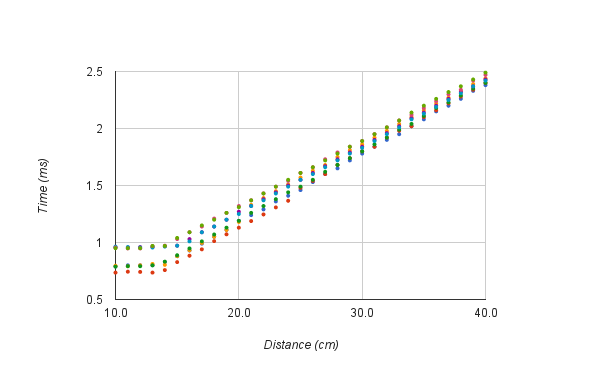
\includegraphics[width=\textwidth]{sonargraph.png}
        \caption{Sonar Test Results}
        \label{fig:sonar_results}
    \end{sidewaysfigure}

    Figure~\ref{fig:software_script} shows the plan developed for testing the sonar driver software.

    \begin{figure}[htb]
        \centering
        \begin{framed}
        \begin{enumerate*}
            \item Connect a computer running Code Composer Studio
            via USB to the debug port of the Tiva board.
            \item In the code that integrates with sonar driver
            \begin{enumerate*}
                \item Send select line signals and print values
                \item Activate trigger signal and print current time
                \item Activate inhibit signal and print current time
                \item Make sure select line is sending correct value
                according to specified order.
                \item Ensure the trigger and inhibit signals
                are activated \SI{0.57}{\milli\second} apart.
                \item Iterate through each select line value
                as shown in Table~\ref{tab:sonar_select}
            \end{enumerate*}
            \item Connect sonar array to Tiva board GPIO
            \item Position selected sonar sensor on ledge
            to prevent surface interference
            \item Using a ruler and object with a flat vertical surface
            \begin{enumerate*}
                \item Place the object such that its surface is orthogonal
                to the sensor
                \item Distance the object beginning at \SI{10.0}{\centi\meter}
                and incrementing by \SI{1.0}{\centi\meter} until
                \SI{40.0}{\centi\meter}
                \item Record the distance
            \end{enumerate*}
            \item In the code that integrates with the sonar driver
            \begin{enumerate*}
                \item Send select line signal and print value
                \item Activate trigger and inhibit signals as described above
                \item Wait for echo interrupt and print resulting value
                \item Calculate distance from value
                and compare to actual distance from sonar.
                \item Iterate through each select line value.
            \end{enumerate*}
            \item Repeat for each incremental distance.
            \item Repeat 8 times for each sensor.
        \end{enumerate*}
        \end{framed}
        \caption{Sonar Driver Test Script}
        \label{fig:software_script}
    \end{figure}

\FloatBarrier
\section{Considerations}
    \label{sec:considerations}
    %chptr 14 notes: DFM, DFA, DFU, failure/reliability, maintainability, sustainability
    
    Because our project is specifically the renovation of a single robot platform,
    many of the standard design considerations are out of project scope. (For instance,
    we do not consider the price viability of using the Raspberry Pi for mass production).
    That being said there are still some important topics to consider as listed here.
    
        \subsection{Design for Manufacturing}

            In order to reduce the manufacturing cost in our project,
            many of the pre-existing components are being retained.
            Particular examples include the chassis, motors, wheels, and sonar array.
            These modules have been tested to perform to project requirements
            and show no reason to be replaced.
    
        \subsection{Design for Assembly}

            Use of the pre-existing chassis simplifies the design
            as there are already points to install sensors, actuators and power supplies.
            In fact, because the chassis is already equipped with motors,
            the only assembly will be done to replace prototyping breadboards 
            with permanent, soldered circuit boards.
            This will be done by hand as a single run labor task.
            Where practical, ``commercial-off-the-shelf'' components have been chosen
            to reduce complexity in assembly and cost.
        
        \subsection{Environmental}
        
            The main environmental concern for our robot is potential pollution
            from the energy source. 
            In our current design, we use a rechargable lead-acid battery.
            The recharable nature allows us to reduce waste generated by single use batteries.
            In addition lead-acid battery recycling
            is one of the most successful recycling programs in the world.
            Retailers that sell batteries collect used batteries for recycling,
            as required by most state laws.
            As such, at the end of the MAVRIC project life cycle,
            the battery should be taken to a local retailer for recycling.
            %citation needed for the recycling program comment?
            % If the citation is wikipedia, then no.
    
        \subsection{Ethical}
        
            It is important to remember that our project is specifically
            to update the hardware inside the MAVRIC system,
            and has only a limited relationship with the driving software
            (which, as an intelligent agent, has a legion of ethical considerations).
            That being said, 
            we can consider the ethical implications of the actuators and sensors
            we render to the robot.
            
                \subsubsection{Privacy}
                
                    An autonomous agent has potential to invade privacy as it collects data.
                    If used as intended, inside a controlled experiemental lab space,
                    there should be no personal data for collection
                    that could cause ethical issues.
                    With its limited sensor space,
                    we conclude this to be true of all sensors onboard MAVRIC.
                
                \subsubsection{Hazards}
                
                    The robot actuators are a pair of DC motors
                    capable of driving at moderate speeds.
                    In order to prevent harmful collisions,
                    we implement a remote stop mechanism, or ``kill switch.''
                    If used in the proper lab space with the stop switch,
                    operational hazards should be minimized.
                
                \subsubsection{Economic}
                
                    As progress continues in computational intelligence,
                    the potential effects on the labor market are severe.
                    Just as the agricultural revolution reduced the man-power required for food
                    and the industrial revolution in many ways commoditized labor,
                    this technological revolution may remove the need
                    for many positions in today's economy.
                    As machines have supplanted many laborers,
                    the economy has moved to value ``knowledge workers.''
                    As computational intelligence matures,
                    decision-making that once only humans could do, may be overtaken by machines.
                    Obviously, this would be very disruptive to the labor market.

    %f. an understanding of professional and ethical responsibility
    %This needs to be addressed in your PDD (Section VIII).
    %Use what you?ve learned in your ethics course(s) to address any 
    %ethical issues associated with your project.

    %h. the broad education necessary to understand the impact of engineering solutions
    % in a global, economic, environmental, and societal context

\clearpage
\FloatBarrier
\section{Project Management} % DONE
    \label{sec:project_management}

        A work breakdown structure
        (shown in Figure~\ref{fig:work_breakdown_structure})
        was developed to identify and clarify the phases of the project.
        A more granular breakdown of the tasks, dependencies, and deadlines
        outlined in the work breakdown structure (Figure~\ref{fig:work_breakdown_structure})
        was developed into a Gantt chart.
        Figure~\ref{fig:gantt} shows the Gantt chart.

        \begin{figure}[htb]
            \begin{framed}
            \centering
            \begin{enumerate*}
                \item Preliminary Work
                \begin{enumerate*}
                    \item Examine problem statement
                    \item Research
                    \item Client interview
                \end{enumerate*}
                \item Zoning In
                \begin{enumerate*}
                    \item Finalize problem statement
                    \item Create full list of objectives and constraints
                    \item Create metrics
                    \item Assign points for metrics
                \end{enumerate*}
                \item Brainstorming design alternatives
                \begin{enumerate*}
                    \item Create morphological chart
                    \item Create candidate designs
                \end{enumerate*}
                \item Design Choice
                \begin{enumerate*}
                    \item Compare design metrics
                    \item Communication with client
                    \item Preliminary testing
                \end{enumerate*}
                \item Prototyping
                \begin{enumerate*}
                    \item Gather materials
                    \item Determine sources and tools
                    \item Delegate responsibility
                    \begin{enumerate*}
                        \item Building
                        \item Programming
                        \item Testing
                        \item Integration
                        \item Documentation
                    \end{enumerate*}
                \end{enumerate*}
                \item Final Report
                \item Colloquium Presentation
                \item Project Management Activities
                \begin{enumerate*}
                    \item Weekly Meetings
                    \item Progress Reports
                    \item Scheduling
                    \item Source Control
                \end{enumerate*}
            \end{enumerate*}
            \end{framed}
            \caption{Work Breakdown Structure}
            \label{fig:work_breakdown_structure}
        \end{figure}

        \begin{sidewaysfigure}[htb]
            \centering
            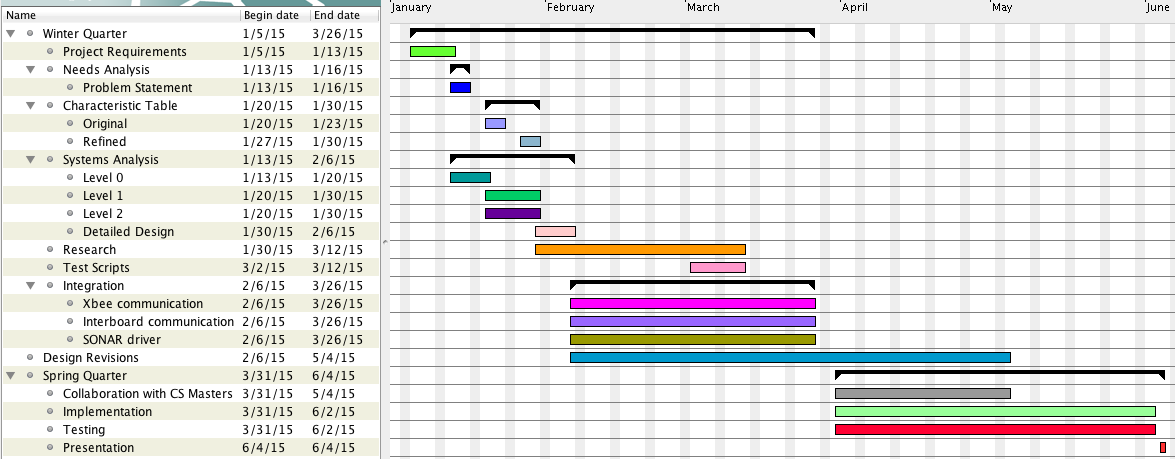
\includegraphics[width=\textwidth]{gantt.png}
            \caption{Schedule}
            \label{fig:gantt}
        \end{sidewaysfigure}

        The budget for the project is outlined in the Bill of Materials
        shown in Table~\ref{tab:bom}.
        An estimated total cost of \SI{229.13}[\$]{} has been identified.
        According to the metrics assigned by equation~\ref{eq:cost},
        this budget earns 6 of 10 points.

        \begin{table}[htb]
            \centering
            {\footnotesize
\begin{tabular}{llrrr}
                                                            &&                  & \textbf{Cost per}     &                       \\
    \multicolumn{2}{l}{\textbf{Item}}                       & \textbf{Count}    & \textbf{Item}         & \textbf{Cost}         \\ \hline
    MAX4466 & electret microphone amplifier                 & 2                 & 16.00                 & 32.00                 \\
    MSGEQ7 & graphic equalizer display filter               & 2                 & 4.95                  & 9.90                  \\
    TM4C1294 LaunchPad & microcontroller board              & 1                 & 19.99                 & 19.99                 \\
    Raspberry Pi B+ & single board computer                 & 1                 & 29.99                 & 29.99                 \\
    ADXL335 & triple axis accelerometer                     & 1                 & 14.99                 & 14.99                 \\
    TSL235 & light-to-frequency converter                   & 3                 & ---                   & ---                   \\
    ATtiny85 & slave microcontroller                        & 1                 & ---                   & ---                   \\
    HC-SR04 & distance sensor                               & 1                 & 5.00                  & 5.00                  \\
    MCC7805 & \SI{5}{\volt} positive voltage regulator      & 1                 & ---                   & ---                   \\
    XBee Pro 900 RPSMA & wireless transceiver               & 2                 & ---                   & ---                   \\
    M891 & leaded NTC thermistor                            & 2                 & ---                   & ---                   \\
    ActivMedia Pioner 2 & chassis                           & 1                 & ---                   & ---                   \\
    PS-1270 & battery                                       & 2                 & ---                   & ---                   \\
    GM9236E132 & \SI{12}{\volt} DC motor                    & 2                 & ---                   & ---                   \\
    VNH5019A & motor controller                             & 2                 & ---                   & ---                   \\
    Wombat (PTH) & prototyping board                        & 4                 & 9.95                  & 39.80                 \\
    \multicolumn{2}{l}{Raspberry Pi Camera Board}           & 1                 & 25.00                 & 25.00                 \\
    FS7548 & flex sensor                                    & 4                 & 12.95                 & 51.80                 \\
    TIP122 & NPN Darlington transistor                      & 1                 & 0.66                  & 0.66                  \\
    \multicolumn{2}{l}{various resistors, capacitors, wire, etc.} & ---               & ---                   & ---                   \\ \hline
    \multicolumn{4}{r}{\textbf{Total}}                                                                  & 229.13                \\ \hline
\end{tabular}
Items without a cost are on hand.
}

            \caption{Bill of Materials}
            \label{tab:bom}
        \end{table}

\FloatBarrier
\section{Research} % DONE (CC)

    \subsection{Library Search Results} % DONE
        \label{sec:research}
        
            Several published works were researched for relevance to our project.
            
            \subsubsection{``A Systems Software Architecture
            For Training Neural Fuzzy Neural
            And Genetic Computational Intelligent Networks''%
            \cite{neural}}
            
                This paper describes a systems approach to neural networking.
                This is similar to the application
                for which our platform is being developed.
                The article in fact references one of Professor Mobus?s
                presentations from 1994 on the subject.
                Though not directly applicable to the scope of our project,
                this article provides context for the system
                in which our platform will be performing.

            \subsubsection{``Design of remote data monitoring
            and recording system Based on ARM''%
            \cite{remote}}

                This article describes the design and implementation
                of a remote sensor system.
                The system shares many characteristics of our own project.
                FreeRTOS is implemented on the ARM architecture
                to poll sensors and then packetize and transmit data.
                The SPI protocol is used.
                Though the targets are different than our own
                (FAT file system instead of POSIX computer),
                the fundamental problem of collecting
                and sending data using FreeRTOS is the same.
                
            \subsubsection{``Interrupt aware Queue Implementation
            for Energy Efficient Multitasking Systems based
            on Cortex-M3 Architecture''
            \cite{cortex}}

                This article addresses means to optimize power efficiency
                when implementing a FreeRTOS application on an ARM Cortex-M system.
                Specifically, a message queue methodology is presented
                for inter-task communication and resource sharing.
                This is relevant to our application
                in that many tasks must run concurrently
                on our Cortex-M4 microcontroller
                and they will need to communicate effectively
                and efficiently on our mobile, battery-powered platform.

        \subsection{Other Research}
        
            The client has written several papers outlining the MAVRIC project history
            which are hosted on his website
            \url{http://faculty.washington.edu/gmobus/AdaptiveAgents/publications.html}.
            These works provide an historical background on the development
            of the MAVRIC platform
            as well as context for its intended experimental research applications.
            
            The documentation from last year's senior design team
            was also reviewed.\cite{mobot}
            This provided insight into the types of problems faced
            in extending the existing platform
            and working with legacy hardware components.
            Specifically, the sonar array presented difficulty for the team.
            This review allowed for anticipation and mitigation of similar difficulties.
            
            Shane Kwon, graduate of the University of Washington Tacoma's
            Master of Science in Computer Science and Systems program,
            shared his research on the MAVRIC.\cite{shane}
            This work thoroughly explains the underlying structure
            of the Adaptrode brain software which will drive the platform.
            This provides guidance on designing the software interface
            created for the Single Board Computer.
            
\section{Concluding Remarks} %TODO
    \label{sec:concluding_remarks}
    
    %ABET, issues to address, as per R. Gutmann:
    
    %i.	a recognition of the need for, and an ability to engage in life-long learning
    %Gutmann: I?m not completely sure how to address this one, but make some mention of 
    %something related to your project that might motivate you to further your education 
    %in a specific area. Maybe you can add a section called ?Concluding Remarks? or
    %?Executive Summary? and include these sorts of comments in there (in addition to other 
    %concluding comments).
        \subsection{Vehicles for Continued Learning}
        
            The MAVRIC project, as expected of a robotic platform, 
            involves many different aspects of engineering.
            Inside, there are several avenues for continued learning.
            
                \subsubsection{FFT's}
                
                    Optimal project implementation would utilize software signal
                    processing through an FFT or a derivative algorithm.
                    Due to time constraints,
                    we have opted to utilize a hardware chip that does this for us.
                    We would nevertheless like to pursue this option and field of study further,
                    even after the project is over,
                    to gain mastery that would enable us to do our own signal processing
                    in later projects.
                
                \subsubsection{Interboard Communication}

                    Communication between distinct components is a pervasive technical challenge.
                    In the MAVRIC project, we had to research the different options
                    and choose one based on our requirements.
                    Mastery of the different communication methods
                    is an interesting and practical endeavor. 
        
                \subsubsection{Artificial Agents and Neural Networks}
                    The area of artificial intelligence (AI) is a vast topic
                    with many interesting aspects.
                    The papers that have been written about MAVRIC encourages 
                    further exploration of neural networks and the current state of AI.
            
    %j.	a knowledge of contemporary issues.
    %Gutmann: In the ?Concluding Remarks? section or, perhaps, in your introduction
    %make some reference to a current issue that impinges on your project.
        \subsection{Contemporary Issues}
        
            Autonomous agents like the MAVRIC robot are rapidly entering our daily lives.
            Self driving cars%
            \footnote{\url{https://plus.google.com/+GoogleSelfDrivingCars/videos}}
            and aerial delivery drones%
            \footnote{\url{http://www.amazon.com/b?node=8037720011}}
            are just two examples of intelligent
            vehicles that will need to operate in a dynamic environment as MAVRIC does.
            Learning behavior will undoubtedly help these agents accomplish their missions.
        
        
\clearpage
\bibliographystyle{plain}
\bibliography{bib.bib}

\end{document}